\documentclass[]{article}

\usepackage{mathtools}
\usepackage{listings}
\usepackage{clrscode}
\usepackage{algorithm}
\usepackage{algorithmic}
\usepackage{graphicx}
\usepackage[top=2cm, bottom=2cm, left=2cm, right=2cm]{geometry}
\DeclareMathOperator*{\argmin}{arg\,min}
\DeclareMathOperator*{\argmax}{arg\,max}

\title{Homework 1}
\date{2015-10-15}
\author{Jingwei Zhang 201528013229095}

\begin{document}
    \maketitle
    \section{Problem 1}
        \subsection{a}
            \paragraph{}Since:
                \begin{align*}
                    P(error|x) = 
                        \begin{cases}
                            P(\omega_2 | x) &\quad \text{if }x>\theta \\
                            P(\omega_1 | x) &\quad \text{if }x \leq \theta
                        \end{cases}
                \end{align*}
            \paragraph{}Then:
                \begin{align*}
                    P(error) &= \int_{-\infty}^{+\infty} p(error,x)  \; \mathrm{d}x \\
                             &= \int_{-\infty}^{\theta} p(\omega_1,x)  \; \mathrm{d}x + \int_{\theta}^{+\infty} p(\omega_2,x)  \; \mathrm{d}x \\
                             &= \int_{-\infty}^{\theta} p(x|\omega_1)P(\omega_1)  \; \mathrm{d}x 
                              + \int_{\theta}^{+\infty} p(x|\omega_2)P(\omega_2)  \; \mathrm{d}x \\
                             &= P(\omega_1)\int_{-\infty}^{\theta} p(x|\omega_1)  \; \mathrm{d}x 
                              + P(\omega_2)\int_{\theta}^{+\infty} p(x|\omega_2)  \; \mathrm{d}x
                \end{align*}
        \subsection{b}
            \paragraph{} Since $x$ is defined on $(-\infty,+\infty)$, if $P(error)$ has minimum, $P'(error)$ must be 0.
                \begin{align*}
                    P'(error) &= [P(\omega_1)\int_{-\infty}^{\theta} p(x|\omega_1)  \; \mathrm{d}x 
                              + P(\omega_2)\int_{\theta}^{+\infty} p(x|\omega_2)  \; \mathrm{d}x]' \\                              
                              &= P(\omega_1)[\int_{-\infty}^{\theta} p(x|\omega_1)  \; \mathrm{d}x ]'
                              - P(\omega_2)[\int_{+\infty}^{\theta} p(x|\omega_2)  \; \mathrm{d}x]' \\                              
                              &= P(\omega_1) p(\theta|\omega_1)
                              - P(\omega_2) p(\theta|\omega_2) \\
                              &= 0
                \end{align*}
            \paragraph{} We can get:
                \begin{equation*}
                    P(\omega_1) p(\theta|\omega_1)
                              = P(\omega_2) p(\theta|\omega_2)
                \end{equation*}
        \subsection{c}
            \paragraph{} No.$P'(error)=0$ for specific $x$ only guarantees that $x$ is an stagnation point. It can be a local maximum, a local minimum or just nothing. And there may be multiple $\theta$ that satisfy the equation.
        \subsection{d}
            \paragraph{}Suppose:
            \begin{align*}
                &P(\omega_1) = P(\omega_2) = \frac{1}{2} \\
                &P(x|\omega_1) = \frac{1}{\sqrt{2\pi}}e^{-(x+1)^2/2} \\
                &P(x|\omega_2) = \frac{1}{\sqrt{2\pi}}e^{-(x-1)^2/2}
            \end{align*}
            \paragraph{} Then:
            \begin{align*}
                &P(error) = \frac{1}{2}\int_{-\infty}^{\theta} \frac{1}{\sqrt{2\pi}}e^{-(x+1)^2/2}  \; \mathrm{d}x 
                              + \frac{1}{2}\int_{-\infty}^{\theta} \frac{1}{\sqrt{2\pi}}e^{-(x-1)^2/2}  \; \mathrm{d}x \\
                &P'(error) =  \frac{1}{2\sqrt{2\pi}}(e^{-(\theta+1)^2/2}+e^{-(\theta-1)^2/2}) \\
                &P''(error) = \frac{-\theta}{\sqrt{2\pi}}(e^{-(\theta+1)^2/2}+e^{-(\theta-1)^2/2})
            \end{align*}
            \paragraph{}So, $P(\omega_1) p(\theta|\omega_1)= P(\omega_2) p(\theta|\omega_2)$($P'(error) = 0$) iff $\theta = 0$.
             And $P''(error)<0, \forall \: \theta \in R$,
             which means that $P'(error) < 0, \forall \: \theta \in (-\infty,0)$ and $P'(error) > 0, \forall \: \theta \in (0,+\infty)$. So that when $\theta = 0$,$P(error)$gets its global maximum.
    \section{Problem 3}
        \subsection{a}
        \paragraph{}Suppose $\mu_1 \leq \mu_2$:
            \subparagraph{}From the probability function we can get that: 
            \begin{align*}
                \begin{cases}
                    p(x|\omega_1) \geq p(x|\omega_1), \text{if } x \leq \frac{\mu_2 + \mu_1}{2} \\
                    p(x|\omega_1) < p(x|\omega_1), \text{if } x > \frac{\mu_2 + \mu_1}{2}
                \end{cases}
            \end{align*}
            \subparagraph{}So, we decide $\omega_1$ if $x \leq (\mu_2 + \mu_1)/2$, otherwise decide $\omega_2$, which minimize $P_e$. Then the probability of error would be:
            \begin{align*}
                P_e &= \int_{-\infty}^{t} p(\omega_2,x)  \; \mathrm{d}x + \int_{t}^{+\infty} p(\omega_1,x)  \; \mathrm{d}x \quad(t=\frac{\mu_2 + \mu_1}{2}) \\
                    &= P(\omega_2)\int_{-\infty}^{t} p(x|\omega_2)  \; \mathrm{d}x + P(\omega_1)\int_{t}^{+\infty} p(x|\omega_1)  \; \mathrm{d}x \\
                    &=\frac{1}{2\sqrt{2\pi}\sigma}(\int_{-\infty}^{t} e^{-\frac{(x-\mu_2)^2}{2\sigma^2}}  \; \mathrm{d}x +\int_{t}^{+\infty} e^{-\frac{(x-\mu_1)^2}{2\sigma^2}}   \; \mathrm{d}x )\\
                    &\text{Let }u_2=\frac{x-\mu_2}{\sigma},
                                u_1=\frac{x-\mu_1}{\sigma} :  \\
                    &=\frac{1}{2\sqrt{2\pi}}(\int_{-\infty}^{\frac{\mu_1 - \mu_2}{2}} e^{-\frac{u_2^2}{2}}  \; \mathrm{d}u_2 +\int_{\frac{\mu_2 - \mu_1}{2}}^{+\infty} e^{-\frac{u_1^2}{2}}   \; \mathrm{d}u_1 )   \\
                    &\text{Let }u=u_1=-u_2 \\ 
                    &=\frac{1}{2\sqrt{2\pi}}(\int_{\frac{\mu_2 - \mu_1}{2}}^{+\infty} e^{-\frac{u^2}{2}}   \; \mathrm{d}u  +\int_{\frac{\mu_2 - \mu_1}{2}}^{+\infty} e^{-\frac{u^2}{2}}   \; \mathrm{d}u ) \\
                    &=\frac{1}{\sqrt{2\pi}}\int_{a}^{+\infty} e^{-\frac{u^2}{2}}   \; \mathrm{d}u \quad (a=\frac{\mu_2 - \mu_1}{\sigma})
            \end{align*}
            \paragraph{}When $\mu_1 > \mu_2$, the process is similar, we can get:
            \begin{align*}
           P_e &=\frac{1}{\sqrt{2\pi}}\int_{a}^{+\infty} e^{-\frac{u^2}{2}}   \; \mathrm{d}u \quad (a=\frac{\mu_1 - \mu_2}{\sigma})
            \end{align*}
            \paragraph{}Above all, the equation$P_e =\frac{1}{\sqrt{2\pi}}\int_{a}^{+\infty} e^{-\frac{u^2}{2}}   \; \mathrm{d}u \quad (a=\frac{|\mu_1 - \mu_2|}{\sigma})$ can be proven.
        \subsection{b}
            \paragraph{}Since:
            \begin{align*}            
            \lim_{a \to \infty} e^{-a^2 /2} = 0 \\
            \lim_{a \to \infty} \frac{1}{\sqrt{2\pi}a} = 0
            \end{align*}
            \paragraph{}We can get:
            \begin{align*}
                \lim_{a \to \infty} P_e &= \lim_{a \to \infty}\frac{1}{\sqrt{2\pi}}\int_{a}^{+\infty} e^{-\frac{u^2}{2}}   \; \mathrm{d}t \\
                    &\leq \lim_{a \to \infty}\frac{1}{\sqrt{2\pi}a}e^{-a^2 /2} \\
                    &=\lim_{a \to \infty} e^{-a^2 /2} \lim_{a \to \infty} \frac{1}{\sqrt{2\pi}a}\\
                    &=0
            \end{align*}
            
    \section{Problem 4}
        \subsection{a}
            \paragraph{} Firstly we can get this probability dense table:
            \begin{table}[h!]
            \centering
            \caption{Probability dense of $p(x_i|\omega_j)$}
            \begin{tabular}{c|*{3}{r}}
                \hline
$p(x_i|\omega_j)$ & $\omega_1$ & $\omega_2$ & $\omega_3$ \\
\hline
$x_1$ & $0.3332$ & $0.3970$ & $0.3683$   \\
$x_2$ & $0.3970$ & $0.3683$ & $0.2661$   \\ 
$x_3$ & $0.2661$ & $0.3683$ & $0.3970$   \\
$x_4$ & $0.2179$ & $0.3332$ & $0.3970$   \\
                \hline
            \end{tabular}
            \end{table}
            \paragraph{} Since these samples are independent, we can get:
            \begin{align*}
P(X|\omega) 
&=P(x_1|\omega_1)P(x_2|\omega_3)P(x3|\omega_3)P(x4|\omega_2)\\
&= 0.01173 \\
            \end{align*}
            \begin{align*}
P(\omega) &=P(\omega_1)P(\omega_3)P(\omega_3)P(\omega_2)\\
&=\frac{1}{128}
            \end{align*}
            \begin{align*}
P(X) 
&= \sum_{\omega_j}P(X,\omega_j) \\
&= \sum_{\omega_j}P(X|\omega_j)P(\omega_j) \\
&= \sum_{j_1=1}^{3} \sum_{j_2=1}^{3}\sum_{j_3=1}^{3}\sum_{j_4=1}^{3} 
   P(x_1|\omega_{j_1})P(\omega_{j_1})P(x_2|\omega_{j_2})P(\omega_{j_2})P(x3|\omega_{j_3})P(\omega_{j_3})P(x4|\omega_{j_4})P(\omega_{j_4})\\
&=0.01208
            \end{align*}
            \paragraph{}Then:
            \begin{align*}
P(\omega|X) 
&=\frac{P(X|\omega)P(\omega)}{P(X)}\\
&=\frac{0.01173/128}{0.01208}\\
&=0.007584
            \end{align*}
        \subsection{b}
            \paragraph{} Similarly:
            \begin{align*}
P(X|\omega) 
&=P(x_1|\omega_1)P(x_2|\omega_2)P(x3|\omega_2)P(x4|\omega_3)\\
&= 0.01793 \\
            \end{align*}
            \begin{align*}
P(\omega) &=P(\omega_1)P(\omega_2)P(\omega_2)P(\omega_3)\\
&=\frac{1}{128}
            \end{align*}
            \paragraph{}$P(X)$ is exactly the same as above, Then:
            \begin{align*}
P(\omega|X) 
&=\frac{P(X|\omega)P(\omega)}{P(X)}\\
&=\frac{0.01793/128}{0.01208}\\
&=0.01160
            \end{align*}
        \subsection{c}
            \paragraph{}Since these points are independent, we will find the following:
            \begin{align*}
\argmax_{\omega}{P(\omega|X)} 
&=\argmax_{\omega}{(P(X|\omega)P(\omega)\frac{1}{P(X)})}\\
&=\argmax_{\omega}{(P(X|\omega)P(\omega))} \\
&=\argmax_{\omega_i}{(P(x_1|\omega_i)P(\omega_i))},\dots,
  \argmax_{\omega_i}{(P(x_4|\omega_i)P(\omega_i))}\\
&=\omega_1,\omega_1,\omega_1,\omega_1 \quad \text{(It represents the sequence)}
            \end{align*}
            \paragraph{}So the sequence is $\omega_1\omega_1\omega_1\omega_1$.


    \section{Problem 5}
        \subsection{a}
            \paragraph{}Since the samples are drawn by successive and independent selections of $\omega_i$ with probability $P(\omega_i)$,we have:
            \begin{align*}
P(z_{ik}|\omega_i) \sim B(1,P(\omega_i)) = P(\omega_i)^{z_{ik}}(1-P(\omega_i))^{1-z_{ik}}
            \end{align*}
            \paragraph{}Since these selections are independent,we have:
            \begin{align*}
P(z_{i1},\dots,z_{in}|P(\omega_i)) 
&= \prod_{k=1}^n P(z_{ik}|P(\omega_i))\\
&= \prod_{k=1}^n P(\omega_i)^{z_{ik}}(1-P(\omega_i))^{1-z_{ik}}
            \end{align*}
        \subsection{b}
            \paragraph{}The log-ML function is:
            \begin{align*}
l(P(\omega_i)) 
&= \ln P(z_{i1},\dots,z_{in}|P(\omega_i)) \\
&= \sum_{k=1}^n (z_{ik}\ln{P(\omega_i)}+(1-z_{ik})\ln{(1-P(\omega_i))}) \\
&= \ln{P(\omega_i)}\sum_{k=1}^n{z_{ik}} + \ln{(1-P(\omega_i))}(n-\sum_{k=1}^n{z_{ik}})
            \end{align*}
            \paragraph{} To maximize $l(P(\omega_i))$, let the derivative of $l$ be $0$:
            \begin{align*}
\frac{\mathrm{d}l(P(\omega_i))}{\mathrm{d}P(\omega_i)} 
&= \frac{\sum_{k=1}^n{z_{ik}}}{P(\omega_i)} - 
   \frac{n-\sum_{k=1}^n{z_{ik}}}{1-P(\omega_i)} \\
&= \frac{ \sum_{k=1}^n{z_{ik}} - nP(\omega_i)}{P(\omega_i)(1-P(\omega_i))} \\
&= 0
            \end{align*}
            \paragraph{}So, we have:
            \begin{align*}
            \sum_{k=1}^n{z_{ik}} - nP(\omega_i) = 0
            \end{align*}
            \paragraph{}Rewrite it, we have:
            \begin{align*}
\hat{P}(\omega_i) = \frac{1}{n}\sum_{k=1}^n{z_{ik}}
            \end{align*}
            
    
    \section{Problem 6}
        \subsection{Key Code}
            \lstinputlisting[language=Python]{P6_key_code.py}
        \subsection{Results}
            \begin{figure}[H]
                \centering
                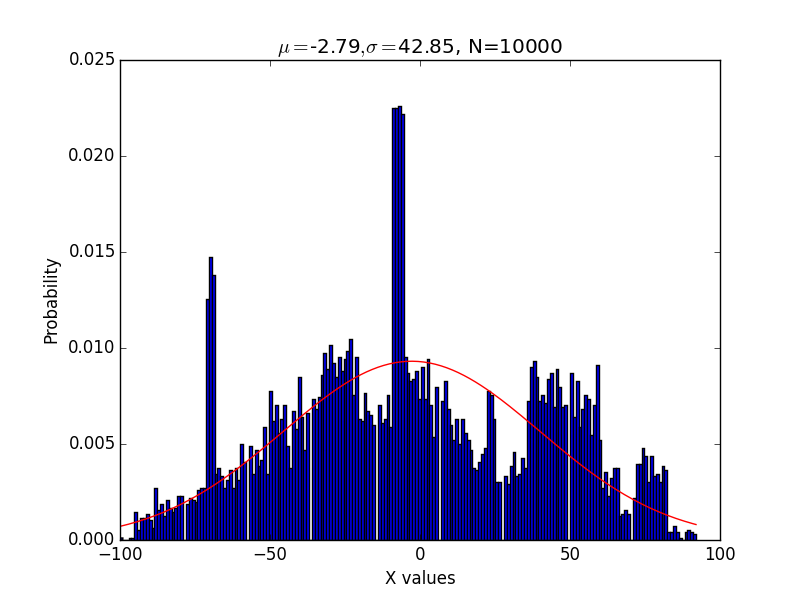
\includegraphics[scale=0.5]{P6_1E4.png}
                \caption{Figure for $10^4$}
            \end{figure}
            \begin{figure}[H]
                \centering
                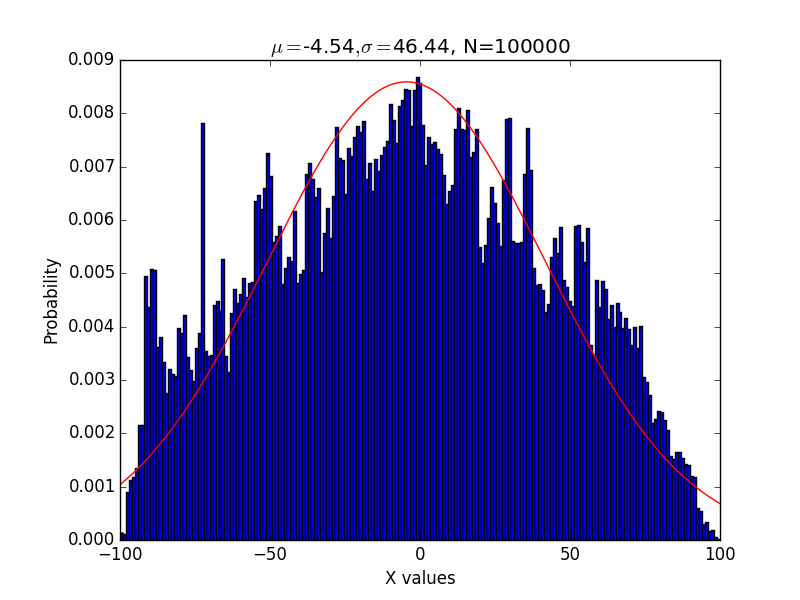
\includegraphics[scale=0.5]{P6_1E5.png}
                \caption{Figure for $10^5$}
            \end{figure}
            \begin{figure}[H]
                \centering
                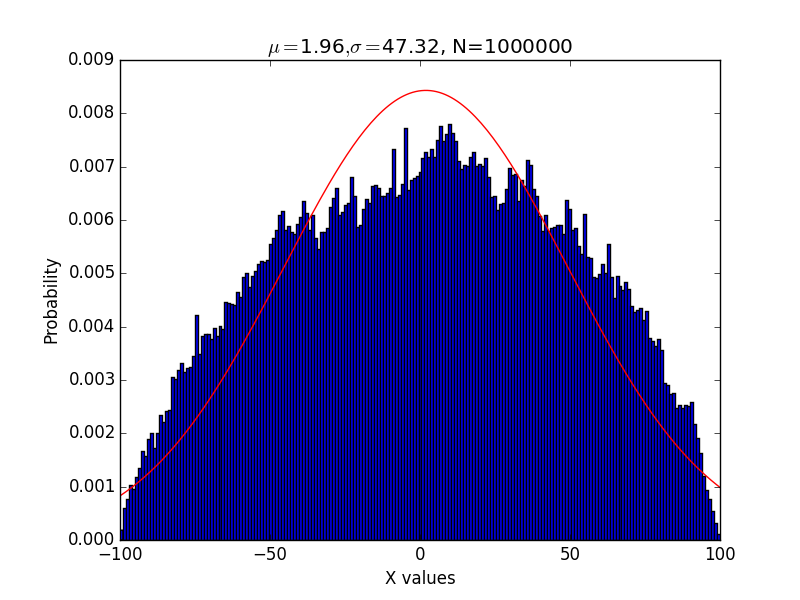
\includegraphics[scale=0.5]{P6_1E6.png}
                \caption{Figure for $10^6$}
            \end{figure}
        \subsection{e) Discuss}
            \paragraph{} It can be seen from above three figures that when the size of sample is small($10^4$), the approximation is not so good.However when the size of sample become larger,as to $10^5$ and $^6$ it is very clear that independent random variables approximate a Gaussian.This illustrate the fact that the approximation can only be applied when the size of sample is sufficiently large.


    \section{Problem 8}
        \subsection{Key Code}
            \lstinputlisting[language=Python]{P8_key_code.py}
        \subsection{Results}
            \paragraph{}Problem a:
            \begin{table*}[h!]
            \centering
            \caption{Problem a: $\mu$ and $\sigma^2$ of $x_i$}
            \begin{tabular}{c|cc}
\hline
$x_i$  &  $\mu$    & $\sigma^2$ \\
\hline            
$x_1$ & $-0.0709$ & $0.90617729$ \\
$x_2$ & $-0.6047$ & $4.20071481$ \\
$x_3$ & $-0.9110$ & $4.54194900$ \\
\hline
            \end{tabular}
            \end{table*}
            \paragraph{}Problem b:
                \subparagraph{}For $(x_1,x_2)$:
                \begin{align*}
                \mu_{12} =(-0.0709,-0.6047) 
                \quad\quad
                \Sigma_{12}  =  \begin{bmatrix}
                    0.90617729 & 0.56778177 \\
                    0.56778177 & 4.20071481 \\
                                \end{bmatrix}
                \end{align*}
                \subparagraph{}For $(x_1,x_3)$:
                \begin{align*}
                \mu_{13} =(-0.0709,-0.9110) 
                \quad\quad
                \Sigma_{13}  =  \begin{bmatrix}
                    0.90617729 & 0.3940801\\
                    0.3940801  & 4.5419490\\
                                \end{bmatrix}
                \end{align*}
                \subparagraph{}For $(x_2,x_3)$:
                \begin{align*}
                \mu_{23} =(-0.6047,-0.9110) 
                \quad\quad
                \Sigma_{23} =  \begin{bmatrix}
                    4.20071481 & 0.7337023\\
                    0.7337023 &  4.541949\\
                                \end{bmatrix}
                \end{align*}
            \paragraph{}Problem c:
                \begin{align*}
                \mu = (-0.0709, -0.6047, -0.911)
                \quad\quad
                \Sigma = \begin{bmatrix}
              0.90617729 & 0.56778177 & 0.3940801 \\
              0.56778177 & 4.20071481 & 0.7337023 \\
              0.3940801  & 0.7337023  & 4.541949  \\
                \end{bmatrix}
                \end{align*}
             \paragraph{}Problem d:
                 \begin{align*}
\mu &= (-0.1126, 0.4299, 0.003720)\\
\Sigma&= diag(0.053925840, 0.045970090, 0.0072655056)
                 \end{align*}
        \subsection{e and f}
            \paragraph{}From result part we find that the corresponding $\mu$ and $\sigma^2$ of $x_i$ are all the same in Problem a,b,c. While in the result of problem b and c, we know that $x1,x2,x3$ are not independent since $\Sigma$ is not a diagonal matrix. This means that the dependency of $x_i$ does not affect their mean and variance because their equations, $\hat{\mu_i} = \frac{1}{n}\sum_{i=1}^n x_i, \hat{Var}(x_i) = \frac{1}{n}\sum_{i=1}^n (x_i-\hat{\mu_i})^2$, have nothing to do with other $x_j(j \neq i)$.
            \paragraph{}Comparing the result we get in problem a,b,c and problem d, their $\mu_i$ and $\sigma_i^2$ are different since they are estimated from different samples of different type $\omega$.


\end{document}